\documentclass[12pt]{article}
\usepackage[a4paper, total={5.5in, 9in}]{geometry}
\usepackage{amsmath}
\usepackage{amsfonts}
\usepackage{graphicx}
\usepackage{enumitem}
\usepackage{hyperref}

\title{Pre-Statistics Worksheet 5}
\author{PCL Learning Center}
\date{}

\begin{document}
\maketitle

\subsection*{Problem 1}
Multiply. Simplify your answer completely:  
\[
\dfrac{32}{5} \cdot \dfrac{16}{56}
\]

\subsection*{Problem 2}
Find three fractions equivalent to the given fraction:  
\[
\dfrac{2}{7}
\]

\subsection*{Problem 3}
Multiply. Write your answer as a simplified fraction or integer:  
\[
-\dfrac{2}{3} \cdot \left(-\dfrac{3}{8}\right)
\]

\subsection*{Problem 4}
Divide. Write your answer as a simplified fraction or integer:  
\[
-\dfrac{4}{7} \div \left(-\dfrac{4}{7}\right)
\]

\subsection*{Problem 5}
Simplify the complex fraction:  
\[
\dfrac{\dfrac{2}{3}}{\dfrac{12}{35}}
\]

\subsection*{Problem 6}
Simplify the complex fraction:  
\[
\dfrac{-4}{\dfrac{7}{3}}
\]

\subsection*{Problem 7}
What fraction of the figure is shaded?  

\begin{figure}[!ht]
    \centering
    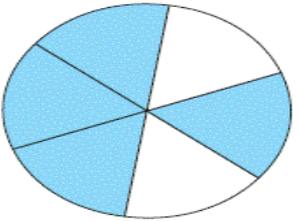
\includegraphics[width=0.5\linewidth]{1.png}
\end{figure}

\begin{itemize}
    \item \textbf{Shaded portion:} \underline{\hspace{3cm}}  
    \item \textbf{Simplest form:} \underline{\hspace{3cm}}
\end{itemize}

\subsection*{Problem 8}
Multiply and simplify:  
\[
\dfrac{3}{16} \cdot \dfrac{8}{15}
\]

\subsection*{Problem 9}
Evaluate the expression and write the result in simplest form.  
(If an answer is undefined, write \textbf{UNDEFINED}.)
\[
\dfrac{5}{8} \div 0
\]

\subsection*{Problem 10}
A space shuttle orbiting Earth travels a distance of about 35 miles in 5 seconds.  
What is the average speed of the space shuttle in miles per second?

\subsection*{Problem 11}
Solve the equation:  
\[
6(y - 2) - 5y = -10
\]

\subsection*{Problem 12}
Solve the equation:  
\[
4x + 8 - 3x + 11 = 20
\]

\subsection*{Problem 13}
Solve the equation:  
\[
7x - 3 = 3x + 9
\]

\subsection*{Problem 14}
Solve the equation:  
\[
2(3y + 1) = 4y + 10
\]

\subsection*{Problem 15}
Solve the equation:  
\[
5x + 2 = 3(x + 4)
\]

\subsection*{Problem 16}
Solve the equation:  
\[
-4(z - 1) + 2z = 3(z - 2)
\]


\section*{Section 2\\ Difficulty level: Hard}
\subsection*{Problem 17}
Simplify the expression completely:
\[
\dfrac{5x - 10}{15x} \div \dfrac{x - 2}{3x^2}
\]

\subsection*{Problem 18}
Solve the equation:  
\[
\dfrac{3x - 7}{5} + \dfrac{2x + 1}{3} = \dfrac{4x - 2}{2}
\]


\end{document}
